\section{III.E. Photomultiplier tubes (PMTs)}

\subsection{Different PMTs time resolutions}
\textit{My assumptions in writing this section}
\begin{enumerate}
	\item \textit{Our chosen PMT(R9779) was compared with panel-1a PMT(EMI9954A)}
	\item \textit {Details of relevant differences of the tech-specs of the two PMTs and therefore the expected superiority of R9779 over EMI9954A will be listed elsewhere; here we will only give empirical proof}
\end{enumerate}

The selected Hamamatusu's R9779 PMTs for panel-1b were compared with Electron Tubes EMI 9954A in the 3-bar setup (\textit{I am assuming that the 3-bar setup will either already be defined or referred to in another publication, so as to not go into details, but simply for the reader to trust that it is our way to extract time-resolution, though, it is NOT directly the time-resolution of the PMT, but of the entire counter; this is important to keep in mind, since for the old TOF system, PMT resolutions were directly compared using lasers; details of this method are in old CLAS-SC NIM paper.})

\textit{Should I mention here that for EMI PMT tests, the contribution of the LFIO module was removed?}

Below is the figure that shows the superiority of the R9779:
\begin{figure}[th]
	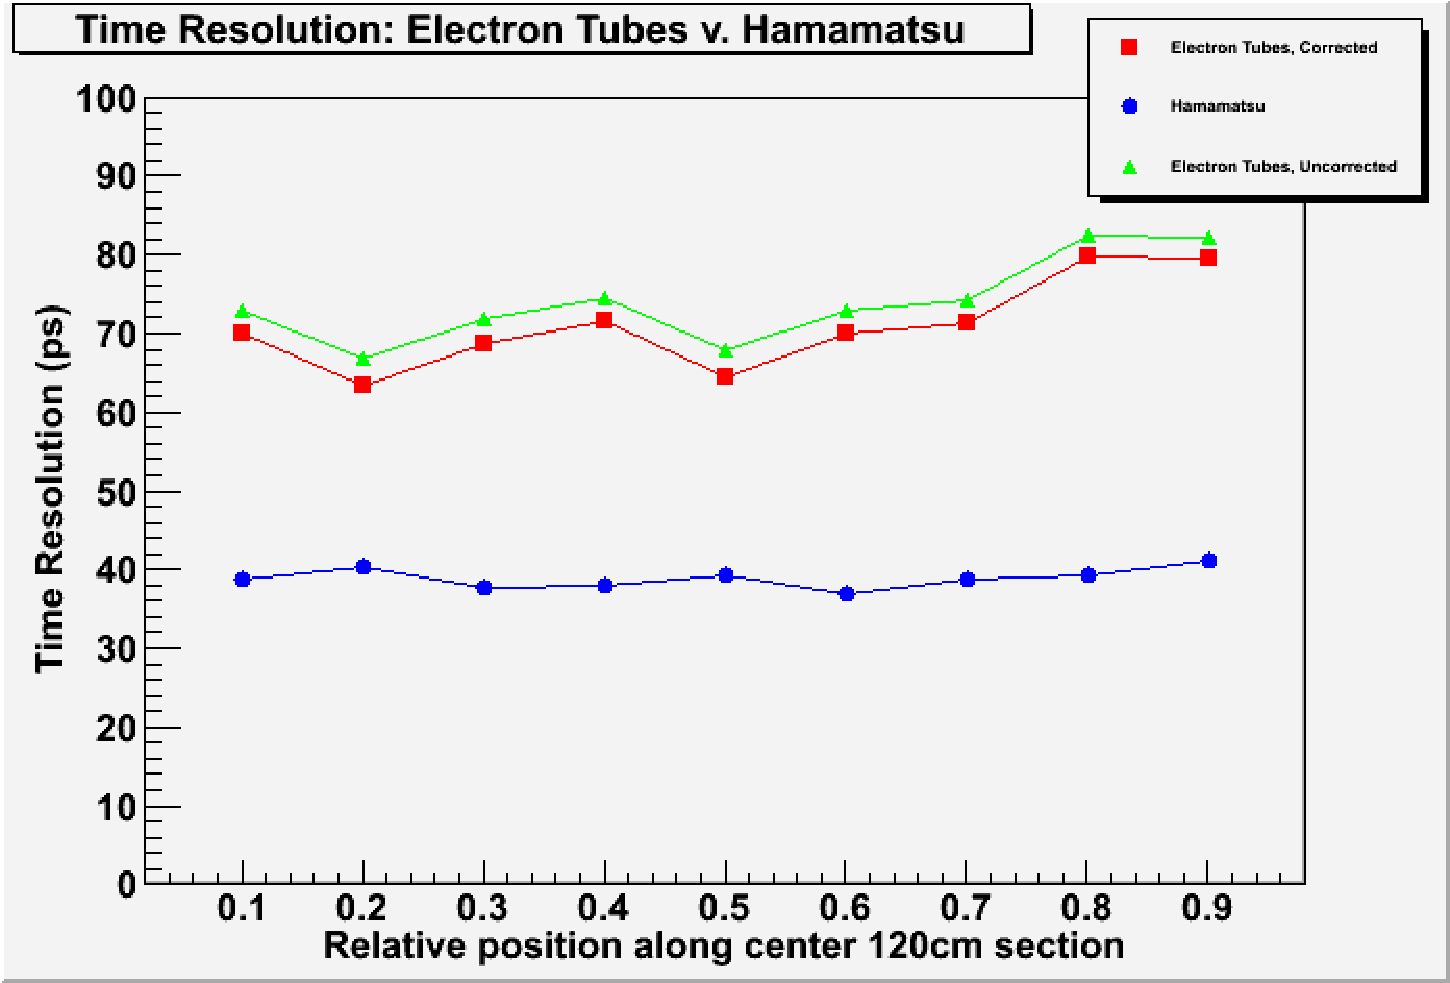
\includegraphics[width=10cm, height=5cm]{arjun/fig_arjun_pmt_resolution/PMTcomparison.pdf}
\end{figure}
